\documentclass[10pt]{article}
\usepackage[usenames]{color} %used for font color
\usepackage{amssymb} %maths
\usepackage{amsmath} %maths
\usepackage{url} %maths
\usepackage[utf8]{inputenc} %useful to type directly diacritic characters
\usepackage{fancyhdr}
% customize fancyhdr package
\pagestyle{fancy} \fancyhf{}
\lhead{
\includegraphics[width=1.5cm]{uni-logo.png}
 \hspace*{.2ex}\parbox[b]{.85\textwidth}{\footnotesize
\hfill   Exercises Week 47 in DM561 / DM562, 2018, IMADA, SDU}}
\rfoot{Page \thepage}

\usepackage{tikz}
\usetikzlibrary{graphs,graphdrawing}
\usegdlibrary{trees, force}
\usepackage{tkz-euclide}
\usetkzobj{all}

\begin{document}
\noindent {\bf Exercise 1: (representations and graph isomorphisms)}\\
Given the following 2 graphs:

 \begin{tikzpicture}[spring layout]    
\tikz [spring electrical layout, node distance=1.3cm,
every edge/.style={
decoration={coil, aspect=-.5, post length=1mm,
segment length=1mm, pre length=2mm},
decorate, draw}]
{
\foreach \i in {1,...,3}
\node (node \i) [fill=blue!30, text=blue!30, circle] {\i};
\draw 
(node 1) edge (node 2) edge (node 3) 
(node 2) edge (node 3);
}
\end{tikzpicture}\hspace{3cm}
 \begin{tikzpicture}[spring layout]    
\tikz [spring electrical layout, node distance=1.3cm,
every edge/.style={
decoration={coil, aspect=-.5, post length=1mm,
segment length=1mm, pre length=2mm},
decorate, draw}]
{
\foreach \i in {1,...,3}
\node (node \i) [fill=blue!30, text=blue!30, circle] {\i};
\draw 
(node 1) edge (node 2)  
(node 2) edge (node 3);
}
\end{tikzpicture}

For each of the graphs, in the following called $G$:
\begin{enumerate}
\item How many different representations (adjacency matrices) can you find for graph $G$? (Let $r_G$ be this number)
\item Chose an adjacency matrix $B$. How many permutation matrices can you find, such that $B=P(PB)^T$? (Let $p_G$  be this number).\\[0.2cm]

  Note: $p_G$ corresponds to the number of isomorphisms from $B$ to itself, which is also called an automorphism. You could chose any pair of representations $A$ and $B$, and finding the number of different $P$ for which $A=P(PB)^T$ holds, the result will always be $p_G$.\\[0.2cm]
\item What is the product of the number of representations $r_G$ and the number of isomorphisms $p_G$? 
\end{enumerate}


\noindent {\bf Exercise 2: (Wiener index and boiling points)}\\
Given the following graph $G$ representing the chemical compound 2,3-dimethylpentan:

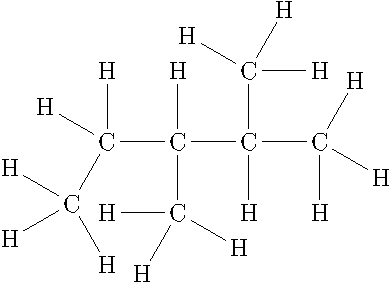
\includegraphics[width=5cm]{23dimethylpentan.pdf}

\begin{enumerate}
\item Determine the edge-weight matrix of the graph of the carbon backbone.
\item Determine the distance matrix.
\item Determine the Wiener-Index.
\item Determine the number of shortest paths of length 3.
\item Determine the value $p_0$ and $w_0$ of the formula for predicting the boiling point for this compound.
\item Determine the estimated boiling points and compare it to the real boiling point.
\item What is the asymptotic worst case performance for finding the distance matrix based on repeated squaring?
\item Do you know a method that has a better asymptotic worst case performance?
\end{enumerate}

\noindent {\bf Exercise 3: (From random polygon to an ellipse)}\\

Given the matrices  \begin{equation*}  M_3 = \frac{1}{2}\left(\begin{array}{ccc}
1 & 1 & 0\\
0 & 1 & 1\\
1 & 0 & 1
\end{array}\right) 
\end{equation*} and \begin{equation*}  M_4 =  \frac{1}{2}\left(\begin{array}{cccc}
1 & 1 & 0 & 0  \\
0 & 1 & 1 & 0  \\
0 & 0 & 1 & 1  \\
1 & 0 & 0 & 1  
\end{array}\right) 
\end{equation*}
\begin{enumerate}
\item Which of both matrices is invertible?
  \item Compute the determinant of $M_3$ and $M_4$.
\item Are the columns of $M_3$ independent? Are the columns of $M_4$ independent?
\item Draw an equilateral triangle with points $(x_1^k, y_1^k)$, $(x_2^k, y_2^k)$, and $(x_3^k, y_3^k)$. Assume the triangle is a result of $M_3\cdot x^{k-1}$ and $M_3\cdot y^{k-1}$ as presented in the lecture. Ignoring normalization, find $x^{k-1}$ and $y^{k-1}$. Can you find several solutions for $x^{k-1}$ and $y^{k-1}$?
\item Draw a square with points $(x_1^k, y_1^k)$, $(x_2^k, y_2^k)$, $(x_3^k, y_3^k)$, and $(x_4^k, y_4^k)$ . Assume the square is a result of $M_4\cdot x^{k-1}$ and $M_4\cdot y^{k-1}$ as presented in the lecture. Ignoring normalization, find $x^{k-1}$ and $y^{k-1}$. Can you find several solutions for $x^{k-1}$ and $y^{k-1}$? What is the conclusion wrt. the (non-)existence of an inverse of $M_4$?
\end{enumerate}

\noindent {\bf Exercise 4: (From random polygons to an ellipse)}\\
 Given vector $v=(0,3,-1,11,-3)$.
\begin{enumerate}
\item Determine $w=v-\overline{v}$, where $\overline{v}$ is a
  vector where each entry is the mean of all values $v_i$.
\item Determine $\frac{w}{||w||_2}$, where $||\cdot||_2$ refers to the 2-norm.
\item What is the length of vector $\frac{w}{||w||_2}$?
\end{enumerate}


\end{document}
%%% Local Variables:
%%% mode: latex
%%% TeX-master: t
%%% End:
